\documentclass[11pt]{article}
\usepackage[margin=2.5cm]{geometry}
\usepackage{amsmath,amssymb}
\usepackage{microtype}
\usepackage{graphicx}
\usepackage[colorlinks=true,linkcolor=blue,citecolor=blue,urlcolor=blue]{hyperref}

\newcommand{\nubar}{\bar\nu}

\title{Secret interactions: couplings, cross sections, and thermal rates}
\author{}
\date{November 2026}

\begin{document}
\maketitle

\noindent
These notes collect the conventions and formulas behind the collision rates of secret interactions in our calculation: how the mediator couples to the mass states (Sec.~\ref{sec:couplings}), the relic neutrinos (Sec.~\ref{sec:relics}), the cross sections on a relic at rest (Sec.~\ref{sec:xsec}), their average over the relics' momenta and, for Dirac neutrinos, their helicity (Sec.~\ref{sec:thermal}), and the four checks (Sec.~\ref{sec:checks}).
We use natural units.

\section{Couplings}
\label{sec:couplings}

A scalar, $\phi$, and a vector, $V$, of mass $M$ couple to neutrinos as
\begin{equation}
 \mathcal{L}_\phi = -\kappa\, \phi \sum_{\alpha\beta} G_{\alpha\beta}\, \bar\nu_\alpha \nu_\beta \;, \qquad
 \mathcal{L}_V = -V_\mu \sum_{\alpha\beta} G_{\alpha\beta}\, \bar\nu_\alpha \gamma^\mu P_L \nu_\beta \;,
\end{equation}
with $\kappa = 1/2$ for Majorana neutrinos and $\kappa = 1$ for Dirac neutrinos, and $G$ a real symmetric matrix in flavor space.
The flavor states are $\nu_\alpha = \sum_i U_{\alpha i} \nu_i$.
In the basis of mass states, the mediators couple through three matrices:
\begin{itemize}
 \item \textit{Scalar, Majorana neutrinos.}
 For Majorana fields, $\nu_\alpha = \sum_i (U_{\alpha i} P_L + U^\ast_{\alpha i} P_R)\, \nu_i$, so
 $\bar\nu_\alpha \nu_\beta = \sum_{ij} \bar\nu_i \left[ (U^T G U)^\ast_{ij} P_R + (U^T G U)_{ij} P_L \right] \nu_j$.
 The mass states couple through the complex symmetric matrix $\lambda = U^T G U$.
 It is real only without CP violation.
 The Majorana phases drop out of every rate; for a single coupled flavor $f$, so does $\delta_{\rm CP}$, since then $|\lambda_{ij}| = g\, |U_{fi}| |U_{fj}|$.
 \item \textit{Scalar, Dirac neutrinos.}
 The coupling is $-\phi \sum_{ij} h_{ij}\, \bar\nu_i \nu_j$, with the Hermitian matrix $h = U^\dagger G U$.
 We give the right-handed neutrinos the same mixing as the left-handed ones.
 \item \textit{Vector, Majorana and Dirac neutrinos.}
 The coupling is through the Hermitian matrix $G' = U^\dagger G U$.
\end{itemize}

The widths of the mediators into neutrinos are
\begin{equation}
 \Gamma_\phi = \frac{M \sum_{kl} |\lambda_{kl}|^2}{16\pi} \;\; \text{(Majorana)} \;, \qquad
 \Gamma_\phi = \frac{M \sum_{kl} |h_{kl}|^2}{8\pi} \;\; \text{(Dirac)} \;, \qquad
 \Gamma_V = \frac{M \sum_{kl} |G'_{kl}|^2}{24\pi} \;.
\end{equation}
Each sum equals ${\rm Tr}(G G^\dagger)$, since $U$ is unitary; for $G = g\, {\rm diag}(0, 0, 1)$ it is $g^2$.

\section{Relic neutrinos}
\label{sec:relics}

The relics of each mass state and each helicity have the number density
\begin{equation}
 n(z) = \frac{3\zeta(3)}{4\pi^2}\, T^3 \;, \qquad T = T_{\nu,0}(1+z) \;, \qquad T_{\nu,0} = 1.676389 \times 10^{-4}~{\rm eV} \;,
\end{equation}
which is $56.0$~cm$^{-3}$ today.
A Majorana relic comes in both helicities.
We sum the cross sections over the relic's spin and multiply them by $n$; equivalently, we average them over the spin and multiply them by $2n$, about $112$~cm$^{-3}$ per mass state today.
A Dirac relic keeps the helicity it had at decoupling: each mass state has $n$ neutrinos of helicity $-1/2$ and $n$ antineutrinos of helicity $+1/2$.
We take the density of relics everywhere as the cosmological mean.

\section{Cross sections on a relic at rest}
\label{sec:xsec}

A high-energy neutrino $\nu_a$, left-handed, of energy $E$, collides with a relic $\nu_r$ of mass $m_r$ at rest, at $s = 2E m_r$.
We write $t = (p_a - p_k)^2$ for the final neutrino $\nu_k$, and $u = -s - t$.

\subsection*{Scalar, Majorana neutrinos}

We take the cross sections of Esteban, Pandey, Brdar \& Beacom, arXiv:2107.13568, Appendix~A, with three changes:
\begin{enumerate}
 \item \textit{Complex couplings.} The appendix takes the couplings real. With $\lambda$ complex, its squared terms take moduli and its interference terms real parts; the $s$--$t$ term, for instance, carries ${\rm Re}[\lambda_{ij}\lambda_{kl}\lambda^\ast_{ik}\lambda^\ast_{jl}]\,(s - M^2)$. The remaining part, proportional to ${\rm Im}[\ldots]\, M\Gamma$, changes sign between neutrinos and antineutrinos, and we leave it out.
 \item \textit{Pair production, $\nu_a \nu_r \to \phi\phi$.} The exchanged neutrino $\nu_k$ enters the amplitude coherently, so the rate carries $|(\lambda\lambda^\dagger)_{ar}|^2$, not the $\sum_k |\lambda_{ak}|^2 |\lambda_{rk}|^2$ printed in Eqs.~(A10), (A11), and (A13). For a single flavor $f$, the printed form is smaller by $\sum_k |U_{fk}|^4$.
 \item \textit{Readings.} The factor $1/2$ of Eq.~(A12) applies only to identical final states, $k = l$. The range of $t$ in pair production is $M^2 - s/2 \mp \sqrt{s(s/4 - M^2)}$.
\end{enumerate}
Summed over the final states, the cross section of $\nu_a$ on $\nu_r$, with the relic's spin summed, is
\begin{equation}
 \label{equ:sigma_scalar}
 \sigma_{ar} = \frac{|\lambda_{ar}|^2 G_2}{16\pi}\,\frac{s}{B}
 + \frac{2 H_{aa} H_{rr} N_2 + |H_{ar}|^2 N_5}{16\pi s}
 + \frac{2\,{\rm Re}(\lambda_{ar} Q_{ar})}{16\pi}\,\frac{(s - M^2) N_4}{B}
 + \frac{|H_{ar}|^2}{32\pi}\, I_{\phi\phi} \;,
\end{equation}
where the four terms are the $s$ channel, the $t$ and $u$ channels, the interference of the $s$ channel with them, and pair production, and
\begin{itemize}
 \item $H = \lambda\lambda^\dagger$, $Q = \lambda^\ast \lambda \lambda^\ast$, $G_2 = \sum_{kl} |\lambda_{kl}|^2$, and $B = (s - M^2)^2 + M^2\Gamma_\phi^2$;
 \item $N_2$, $N_4$, and $N_5$ are the integrals over $x \in [0, 1]$ of $(1-x)^2/(1-x+\mu)^2$, $(1-x)/(1-x+\mu)$, and $x(1-x)/[(x+\mu)(1-x+\mu)]$, with $\mu = M^2/s$; in closed form, with $r = s/M^2$,
 $N_2 = 1 + 1/(1+r) - 2\ln(1+r)/r$, $N_4 = [r - \ln(1+r)]/r$, and $N_5 = 1 - 2(1+r)\ln(1+r)/[r(2+r)]$;
 \item $I_{\phi\phi} = (s - 2M^2)\, \Phi(w)/s^2$ above $s = 4M^2$ and zero below, with $\Phi(w) = 2(3 - w^2)\,{\rm artanh}\, w - 6w$ and $w = \sqrt{s(s - 4M^2)}/(s - 2M^2)$.
\end{itemize}

\subsection*{Scalar, Dirac neutrinos}

The total cross section on a relic at rest is Eq.~(A8) of arXiv:2107.13568, with $h$ in place of the couplings.
The scalar flips chirality at each vertex, so part of the products are sterile; Sec.~\ref{sec:thermal} gives which part of the relic takes part in which channel.

\subsection*{Vector}

For a relic of fixed helicity, $d\sigma/dt = |\mathcal{M}|^2/(16\pi s^2)$, with
\begin{itemize}
 \item a relic that acts as an antineutrino (helicity $+1/2$), $\nu_a \nubar_r \to \nu_k \nubar_l$ through the $s$ and $t$ channels:
 $|\mathcal{M}|^2 = 4u^2 \left| A_s/(s - M^2 + iM\Gamma_V) + A_t/(t - M^2) \right|^2$, with $A_s = G'_{ra} G'_{kl}$ and $A_t = G'_{ka} G'_{rl}$;
 \item a relic that acts as a neutrino (helicity $-1/2$), $\nu_a \nu_r \to \nu_k \nu_l$ through the $t$ and $u$ channels:
 $|\mathcal{M}|^2 = 4s^2 \left| A_t/(t - M^2) + A_u/(u - M^2) \right|^2$, with $A_t = G'_{ka} G'_{lr}$ and $A_u = G'_{la} G'_{kr}$, and a factor $1/2$ for $k = l$;
 \item pair production on a relic that acts as an antineutrino, $\nu_a \nubar_r \to VV$, with
 \begin{equation*}
 |\mathcal{M}|^2 = 4\, |(G' G'^\dagger)_{ar}|^2 \left[ \frac{t}{u} + \frac{u}{t} + \frac{4M^2 s}{tu} - M^4 \left( \frac{1}{t^2} + \frac{1}{u^2} \right) \right] ,
 \end{equation*}
 which integrates, with the factor 1/2 for identical vectors, to $\sigma_{VV} = |(G' G'^\dagger)_{ar}|^2\, I_{VV}/(8\pi)$ above $s = 4M^2$, with
 \begin{equation*}
 I_{VV} = \frac{1}{s^2} \left[ \frac{2(s^2 + 4M^4)\,\Lambda}{s - 2M^2} - 4\sqrt{s(s - 4M^2)} \right] , \qquad
 \Lambda = 2\ln\frac{s - 2M^2 + \sqrt{s(s - 4M^2)}}{2M^2} \;.
 \end{equation*}
\end{itemize}
A Majorana relic offers both kinds, $n$ of each per mass state.

\section{Thermal average and the helicity of Dirac relics}
\label{sec:thermal}

A relic of energy $E_p$ and momentum $p$ that meets the high-energy neutrino at an angle $\theta$ gives $s = m_r^2 + 2E\epsilon$, with $\epsilon = E_p - p\cos\theta$.
Every product of a collision is boosted along the incoming neutrino by a Lorentz factor of about $E/\sqrt{s}$, so its share of the energy is the same in the relic's frame as in the cosmological one, and the cross sections depend on $s$ alone.
With Fermi--Dirac momenta at temperature $T$, isotropic directions, and the flux factor $1 - v\cos\theta$, the distribution of $\epsilon$ is
\begin{equation}
 \rho(\epsilon) = \frac{\epsilon}{3\zeta(3)\, T^3} \int_{p_X}^\infty \frac{p\, f(p/T)}{E_p}\, dp \;, \qquad
 p_X = \frac{X^2 - m_r^2}{2X} \;, \qquad X = \max(\epsilon, m_r^2/\epsilon) \;,
\end{equation}
with $f(y) = 1/(e^y + 1)$.
It is normalized to one, has a kink at $\epsilon = m_r$, and becomes $\delta(\epsilon - m_r)$ for slow relics.
The rate of collisions of $\nu_a$ on the Majorana relic $\nu_r$ is then
\begin{equation}
 \label{equ:rate}
 \Gamma_{ar}(E, z) = n(z) \int d\epsilon\; \rho(\epsilon)\, \sigma_{ar}(s = 2E\epsilon) \;,
\end{equation}
with $\sigma_{ar}$ summed over the relic's spin and over the final states, $E$ the energy at redshift $z$, and the term $m_r^2$ in $s$ neglected.

\subsection*{Dirac relics}

A moving Dirac relic keeps its helicity.
Its spin along the direction of the incoming neutrino is
\begin{equation}
 \pi = \frac{E_p\, \epsilon - m_r^2}{p\, \epsilon} \;,
\end{equation}
from $-1$ for a relic that moves along with the incoming neutrino to $+1$ for one that moves against it.
After averaging over the azimuth of the final state, the squared amplitude is
\begin{equation}
 |\mathcal{M}|^2 = \frac{1+\pi}{2}\, |\mathcal{M}_L|^2 + \frac{1-\pi}{2}\, |\mathcal{M}_R|^2 \;,
\end{equation}
up to terms of order $m_r^2/s$, where $\mathcal{M}_L$ and $\mathcal{M}_R$ are the amplitudes for a massless relic of left- or right-handed chirality at the same $s$; for the antineutrino, the weights apply to the chirality of its spinor $v$.
The two chiral parts of the relic are then distributed as
\begin{align}
 \rho_L(\epsilon) &= \rho\, \frac{1+\pi}{2} = \frac{1}{3\zeta(3)\, T^3} \int_{p_X}^\infty f(p/T)\, \frac{(E_p + p)(\epsilon - E_p + p)}{2E_p}\, dp \;, \\
 \rho_R(\epsilon) &= \rho\, \frac{1-\pi}{2} = \frac{1}{3\zeta(3)\, T^3} \int_{p_X}^\infty f(p/T)\, \frac{(E_p - p)(E_p + p - \epsilon)}{2E_p}\, dp \;.
\end{align}
At rest, each is $\rho/2$.
\begin{itemize}
 \item \textit{Vector.} It couples only to the left-chiral part. The rate is Eq.~(\ref{equ:rate}) with $\rho_L$ in place of $\rho$ and the Majorana cross section of Sec.~\ref{sec:xsec}; at rest, it is half the Majorana rate.
 \item \textit{Scalar.} Every vertex flips chirality, and the daughter of the incoming neutrino is always sterile. The left-chiral part of the relic takes part in $\nu\nu \to \nu\nu$ through the $t$ and $u$ channels together (both final neutrinos sterile), in $\nu\nubar \to \nu\nubar$ through the $t$ channel alone (both sterile), and in pair production. The right-chiral part takes part in $\nu\nu \to \nu\nu$ through the $t$ or the $u$ channel apart (the relic's partner visible), and in $\nu\nubar \to \nu\nubar$ through the $s$ and $t$ channels. The rate is $n \int d\epsilon\, [\rho_L\, \sigma_L + \rho_R\, \sigma_R]$, with $\sigma_{L,R}$ the cross sections on a massless relic of either chirality, summed over the relic neutrino and antineutrino. Thus the $s$-channel resonance needs the right-chiral part, whose share on a relativistic relic is small.
\end{itemize}

\section{The four checks}
\label{sec:checks}

Common to all: $G = g\, {\rm diag}(0, 0, 1)$ with $g = 10^{-3}$, $M = 1$~MeV, the NuFIT~6.1 best fit in normal ordering ($\sin^2\theta_{12} = 0.3088$, $\sin^2\theta_{13} = 0.02248$, $\sin^2\theta_{23} = 0.470$, $\delta_{\rm CP} = 212^\circ$), a lightest mass $m_1 = 10^{-6}$~eV, $z = 0$, and $T_{\nu,0}$ as in Sec.~\ref{sec:relics}.
The quantity is the rate $\Gamma_{31}(E)$ (s$^{-1}$) of an incoming $\nu_3$ on the relic $\nu_1$, for $E$ from 10~TeV to 100~PeV, at 50 log-spaced points per decade, in four cases:
\begin{enumerate}
 \item[A.] Scalar, Majorana.
 \item[B.] Vector, Majorana.
 \item[C.] Scalar, Dirac, with the relics' helicity; also the rates at which the collisions produce active and sterile neutrinos, each the collision rate weighted by the number of active or sterile neutrinos among the products.
 \item[D.] Vector, Dirac, with the relics' helicity.
\end{enumerate}

Figure~\ref{fig:checks} shows our results for the four checks, as the mean free path $c/\Gamma_{31}$ of the incoming $\nu_3$.
We computed each rate from Eq.~(\ref{equ:rate}), with the cross sections of Sec.~\ref{sec:xsec} and the distributions $\rho$, $\rho_L$, and $\rho_R$ of Sec.~\ref{sec:thermal}, by direct quadrature over $\epsilon$.
The broad dip is the $s$-channel resonance.
The relic $\nu_1$ moves almost at the speed of light, so the resonance sits where $2E\epsilon = M^2$ with $\epsilon$ of order $T$, far below the energy $M^2/2m_1$ at which it would sit for a relic at rest.
The vector gives the same rates for Dirac and Majorana neutrinos here, because a relic this fast is almost entirely left-chiral.
For the same reason, the resonance of the scalar with Dirac neutrinos, which needs the right-chiral part of the relic, is much weaker.

\begin{figure}[t]
 \centering
 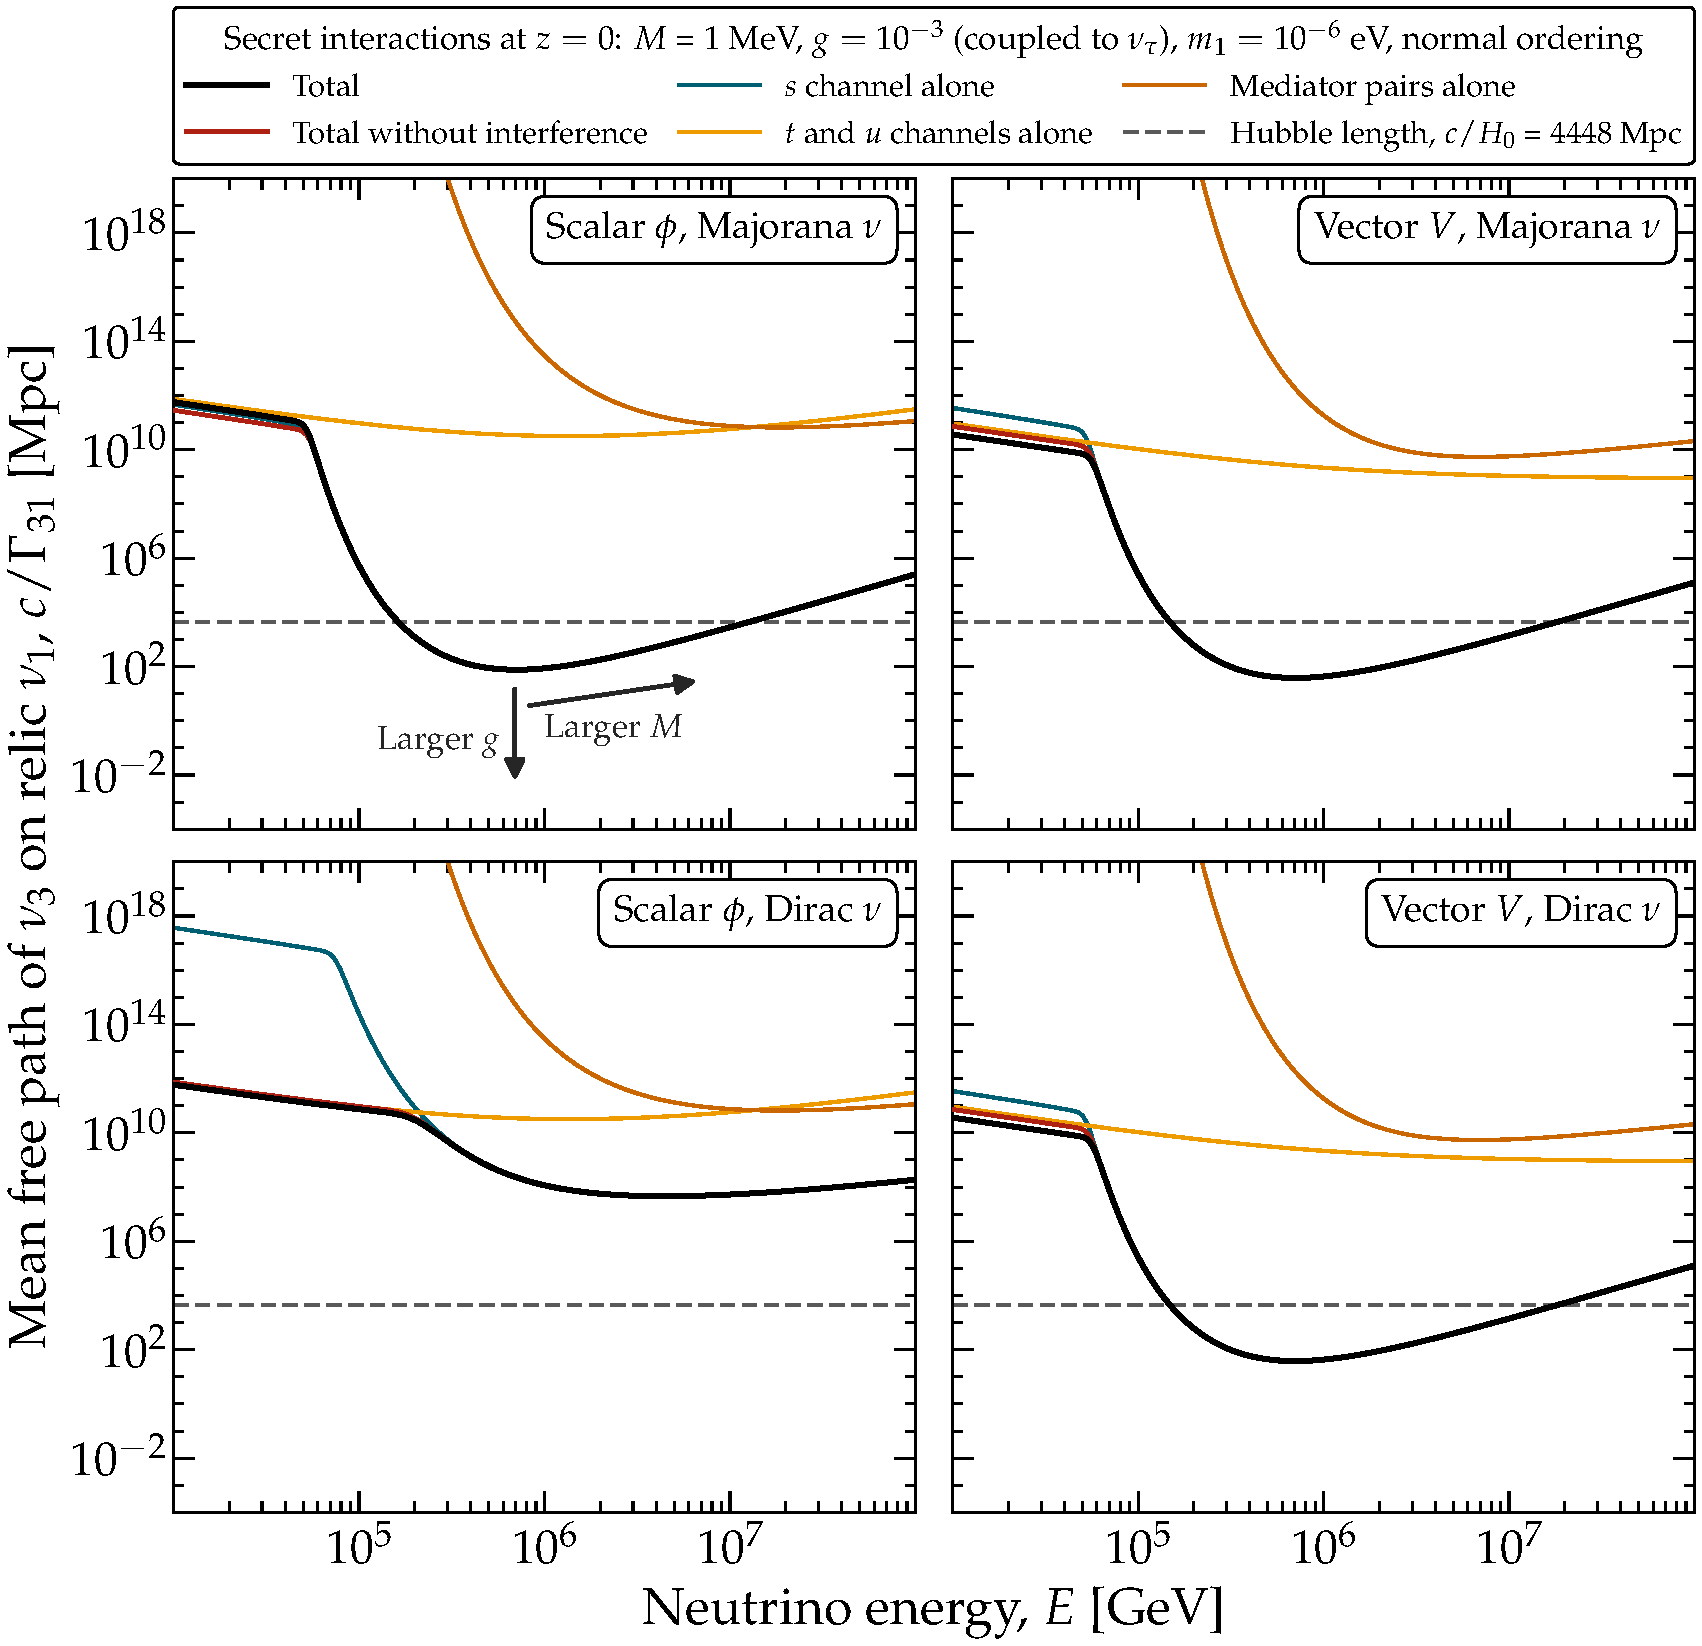
\includegraphics[width=0.92\textwidth]{benchmark_mean_free_paths.pdf}
 \caption{\textbf{\textit{Mean free path of an incoming $\nu_3$ on the relic $\nu_1$, for the four checks.}}
  Left to right and top to bottom, the panels are checks A, B, C, and D, at the common benchmark point above.
  The channel curves leave out the interference terms, which enter only the totals.
  The arrows show schematically how the dip moves for a larger mediator mass $M$ or coupling $g$.}
 \label{fig:checks}
\end{figure}

\end{document}
